\hyphenation{Permanent-magneten}
\section{Ziel}
\label{sec:Ziel}
Ziel des Versuchs ist die Bestimmung des magnetischen Moments eines Permanentmagneten unter Verwendung zweier unterschiedlicher Methoden. Die Ergebnisse dienen anschließend
für einen Vergleich der Genauigkeit der beiden Messmethoden.

\section{Theorie}
\label{sec:Theorie}
\subsection{Einführung}
\label{subsec:Einführung}
Die elementarste Gestalt des Magnetismus ist der magnetische Dipol. Magnetische Monopole gibt es nicht. Da nur Monopole zu Quellen der Feldlinien führen,
müssen Magnetfeldlinien immer geschlossen sein. \\
Zur Untersuchung von Dipolen eignen sich Permanentmagneten oder geschlossene, stromdurchflossene Leiterschleifen, da diese sich mikroskopisch
wie magnetische Dipole verhalten. Das magnetische Moment $\vec{\mu}_{\text{Dipol}}$ ist eine wichtige Größe in der Magnetostatik und der Elektrodynamik, dass zur Beschreibug der
Stärke eines magnetischen Dipols genutzt werden kann. Das magnetische Moment einer stromdurchflossenen Leiterschleife kann durch 
\begin{equation}
\label{eqn:mu Leiterschleife}
    \vec{\mu} = I \cdot \vec{A}
\end{equation}
berechnet werden, wobei $I$ der Strom und $\vec{A}$ die orientierte Querschnittsfläche der Leiterschleife ist. \\

\subsection{Drehmomente auf Körper im Gravitations- und Magnetfeld}
\label{subsec:Drehmomente}
Das magnetische Moment eines Permanentmagneten kann nur experimentell bestimmt
werden. Dazu wird häufig eine makroskopischer magnetischer Dipol in einem homogenen Magnetfeld betrachtet. Befindet sich ein Dipol im Magnetfeld, so wirkt dieses ein Drehmoment
auf den Dipol aus. Dieses Drehmoment richtet den Dipol parallel zu den Feldlinien aus. Im homogenen Magnetfeld $\vec{B}$ wirkt das Drehmoment $\vec{D}_{\text{B}}$ mit: 
\begin{equation}
    \label{eqn:Drehmoment B-Feld}
    \vec{D}_{\text{B}} = \vec{\mu}_{\text{Dipol}} \times \vec{B}
\end{equation}
In einem Teil des Versuches ist ein weiteres Drehmoment relevant. Dieses wirkt auf einen drehbar gelagerten Körper, sofern das Objekt nicht bereits parallel zum 
Schwerefeld $\vv{F}_{\text{G}}$ ausgerichtet ist und sich der Schwerpunkt nicht auf der Drehachse befindet. Das Drehmoment $\vec{D}_{\text{G}}$ ergibt sich mit der
Erdbeschleunigung $\vv{g}$ und dem Verbindungsvektor von Drehachse und Schwerpunkt $\vv{r}$ zu:
\begin{equation}
    \label{eqn:Drehmoment Schwerefeld}
    \vec{D}_{\text{G}} = m(\vv{r} \times \vv{g})
\end{equation}
Falls sich ein Gleichgewicht zwischen diesen Drehmomenten einstellt ergibt sich die Formel:
    \begin{align*}
    \label{eqn:Drehmoment_Gleichgewicht}
    \vec{D}_{\text{B}} &= \vec{D}_{\text{G}} \\
    \Leftrightarrow \vec{\mu}_{\text{Dipol}} \times \vec{B} &= m(\vv{r} \times \vv{g})
\end{align*}
Man kann das Kreuzprodukt dann mit der allgemeinen Formel 
\begin{equation}
    \label{eqn:Kreuzprodukt}
    \vec{A} \times \vec{B} = \sin(\sphericalangle(\vec{A},\vec{B}))\lvert A \rvert \cdot\lvert B \rvert
\end{equation}
umschreiben. So erhält man
\begin{equation}
    \label{eqn:Drehmoment_Gleichgewicht1}
    \mu_{\text{Dipol}}\cdot B\cdot \sin\theta = m\cdot r\cdot g\cdot\sin\theta
\end{equation}
Nach kürzen von $\sin\theta$ und umstellen auf $\mu_{\text{Dipol}}$ erhält man schließlich den Ausdruck
\begin{equation}
    \label{eqn:Drehmoment_Gleichgewicht2}
    \mu_{\text{Dipol}} = \frac{m \cdot r\cdot g}{B} 
\end{equation}

\subsection{Erzeugung homogener Magnetfelder}
\label{subsec:HomogeneMagnetfelder}
Homogene Magnetfelder kommen nie natürlich vor. Allerdings lassen sich hinreichend homogene Magnetfelder konstruieren. Dies kann durch ein Helmholtzspulenpaar realisiert werden.
\begin{figure}
	\centering
    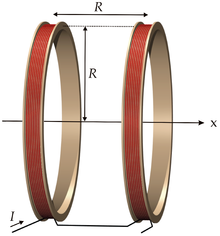
\includegraphics[width=0.4\textwidth]{content/Helmholtz_coils.png}
	\caption{Skizze eines Helmholtzspulenpaares \cite{Helmholtzspulenpaar}.}
	\label{fig:Helmholtzspulenpaar}
\end{figure}
Durch die Anordnung der Spulen in \autoref{fig:Helmholtzspulenpaar} bildet sich in der Mitte zwischen den beiden Spulen ein homogenes Magnetfeld entlang der Symetrieachse, welches 
jedoch nach außen inhomogener wird. Die Spulen müssen gleichsinnig vom Strom durchlaufen werden und der Radius der Spulen muss dem Abstand der beiden Spulen entsprechen. 
Das Magnetfeld entlang der Symetrieachse für Spulen mit je einer Windung kann über das Biot-Savart-Gesetz
\begin{equation}
    \label{eqn:diff_Biot-Savart}
    d\vv{B} = \frac{\mu_0 I}{4\pi}\frac{d\vec{s}\times\vec{r}}{r^3}
\end{equation}
nach Integration durch
\begin{equation}
    \label{eqn:Biot-Savart_1}
    \vv{B}(x) = \frac{\mu_0 I}{2}\frac{R^2}{\left(R^2 + x^2 \right)^{(3/2)}}\cdot \vec{e}_x
\end{equation}
berechnet werden. Hierbei wir die Symetrieachse als x-Achse definiert (vgl. \autoref{fig:Helmholtzspulenpaar1}). Das \dq x\dq \: entspricht hier dem halben Abstand der beiden Spulen. 
\begin{figure}
	\centering
    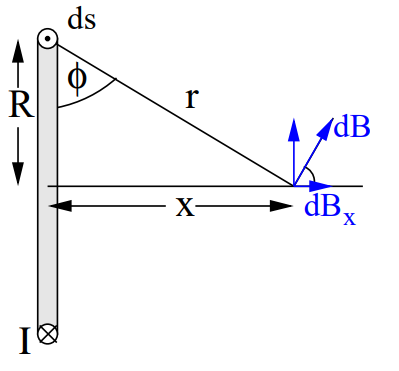
\includegraphics[width=0.4\textwidth]{content/Helmholtzachsen.PNG}
	\caption{Ergänzungsskizze der Achsen zum Helmholtzspulenpaares  \cite{v105}.}
	\label{fig:Helmholtzspulenpaar1}
\end{figure}
Das Magnetfeld im inneren des Helmholtzspulenpaares lässt sich nun durch Überlagerung der Einzelfelder bestimmen. Der Ursprung der gewählten Koordinaten wird dafür in die Mitte 
gesetzt und es werden pro Spule $N$ Windungen betrachtet. Daher ergibt sich das Magnetfeld an dieser Stelle zu
\begin{equation}
    \label{eqn:Helmholtz_B}
    B(0) = N\cdot B(-x) +N\cdot B(x) = \frac{N\mu_0 IR^2}{\left(R^2 + x^2 \right)^{(3/2)}}
\end{equation}

\subsection{Schwingung eines Dipols}
\label{subsec:Schwingung}
In einem weiteren Teil des Versuchs wird das magnetische Dipolmoment $\vv{\mu}_{\text{Dipol}}$ über die Messung der Schwingungsdauer eines Dipols, welcher im homogenen Magnetfeld
in Schwingung versetzt wird, bestimmt. Da sich ein schwingender Dipol im homogenen Magnetfeld wie ein harmonische Oszillator verhält, kann man dessen Bewegung beschreiben durch
\begin{equation}
    \label{eqn:BewegungsgleichungKugel}
    -\lvert \vv{\mu}_{\text{Dipol}} \times \vv{B}\rvert = J_{\text{K}} \cdot \frac{d^2 \theta}{dt^2}
\end{equation}
Diese Differentialgleichung zweiter Ordnung wird gelöst durch die Schwingungsdauer $T$. $T$ ist dabei bestimmt durch
\begin{equation}
    \label{eqn:Schwingungsdauer}
    T^2 = \frac{4{\pi}^2 J}{{\mu}_{\text{Dipol}}}\frac{1}{B}
\end{equation} 
$J$ ist das Trägheitsmoment des Körpers. Das Trägheitsmoment beschreibt die Trägheit eines rotierenden Körpers gegenüber der Änderung seiner Winkelgeschwindigkeit.
Allgemein gilt für $J$ die Formel:
\begin{equation}
    \label{eqn:Trägheitsmoment}
    J = \int_{\text{V}} {r^2}_{\bot} \text{d}m = \int_{\text{V}} {r^2}_{\bot} \rho \text{d}V
\end{equation} 
\cite{Demtröder_Exp_P_1}
Für den Spezialfall einer Kugel ergibt sich diese Formel zu:
\begin{equation}
    \label{eqn:Trägheitsmoment_Kugel}
    J_{\text{K}} = \frac{2}{5} m R^2
\end{equation}
